% !TEX root = paper.tex

\section {Results}
\label{sec:results}

\subsection{Ridge yield}

Measurement of the correlations function is shown in Fig.~\ref{fig:PlotCorrMBHMT} for 1.0$<\it{p}_{\rm{T, assoc}},\,\it{p}_{\rm{T, trig}}<$2.0 GeV/\it{c}\rm{} in pp collisions at $\sqrt{\it{s}} = $\unit{13} {\rm{}TeV} in the 0-0.1\% (left), and 0-100\% (right) multiplicity class estimated by V0 detector, which covers forward rapidity region. The ridge is clearly seen in high multiplicity class unlike in lower multiplicity classes.

\begin{figure}[h!]
	\centering
	\subfigure{ 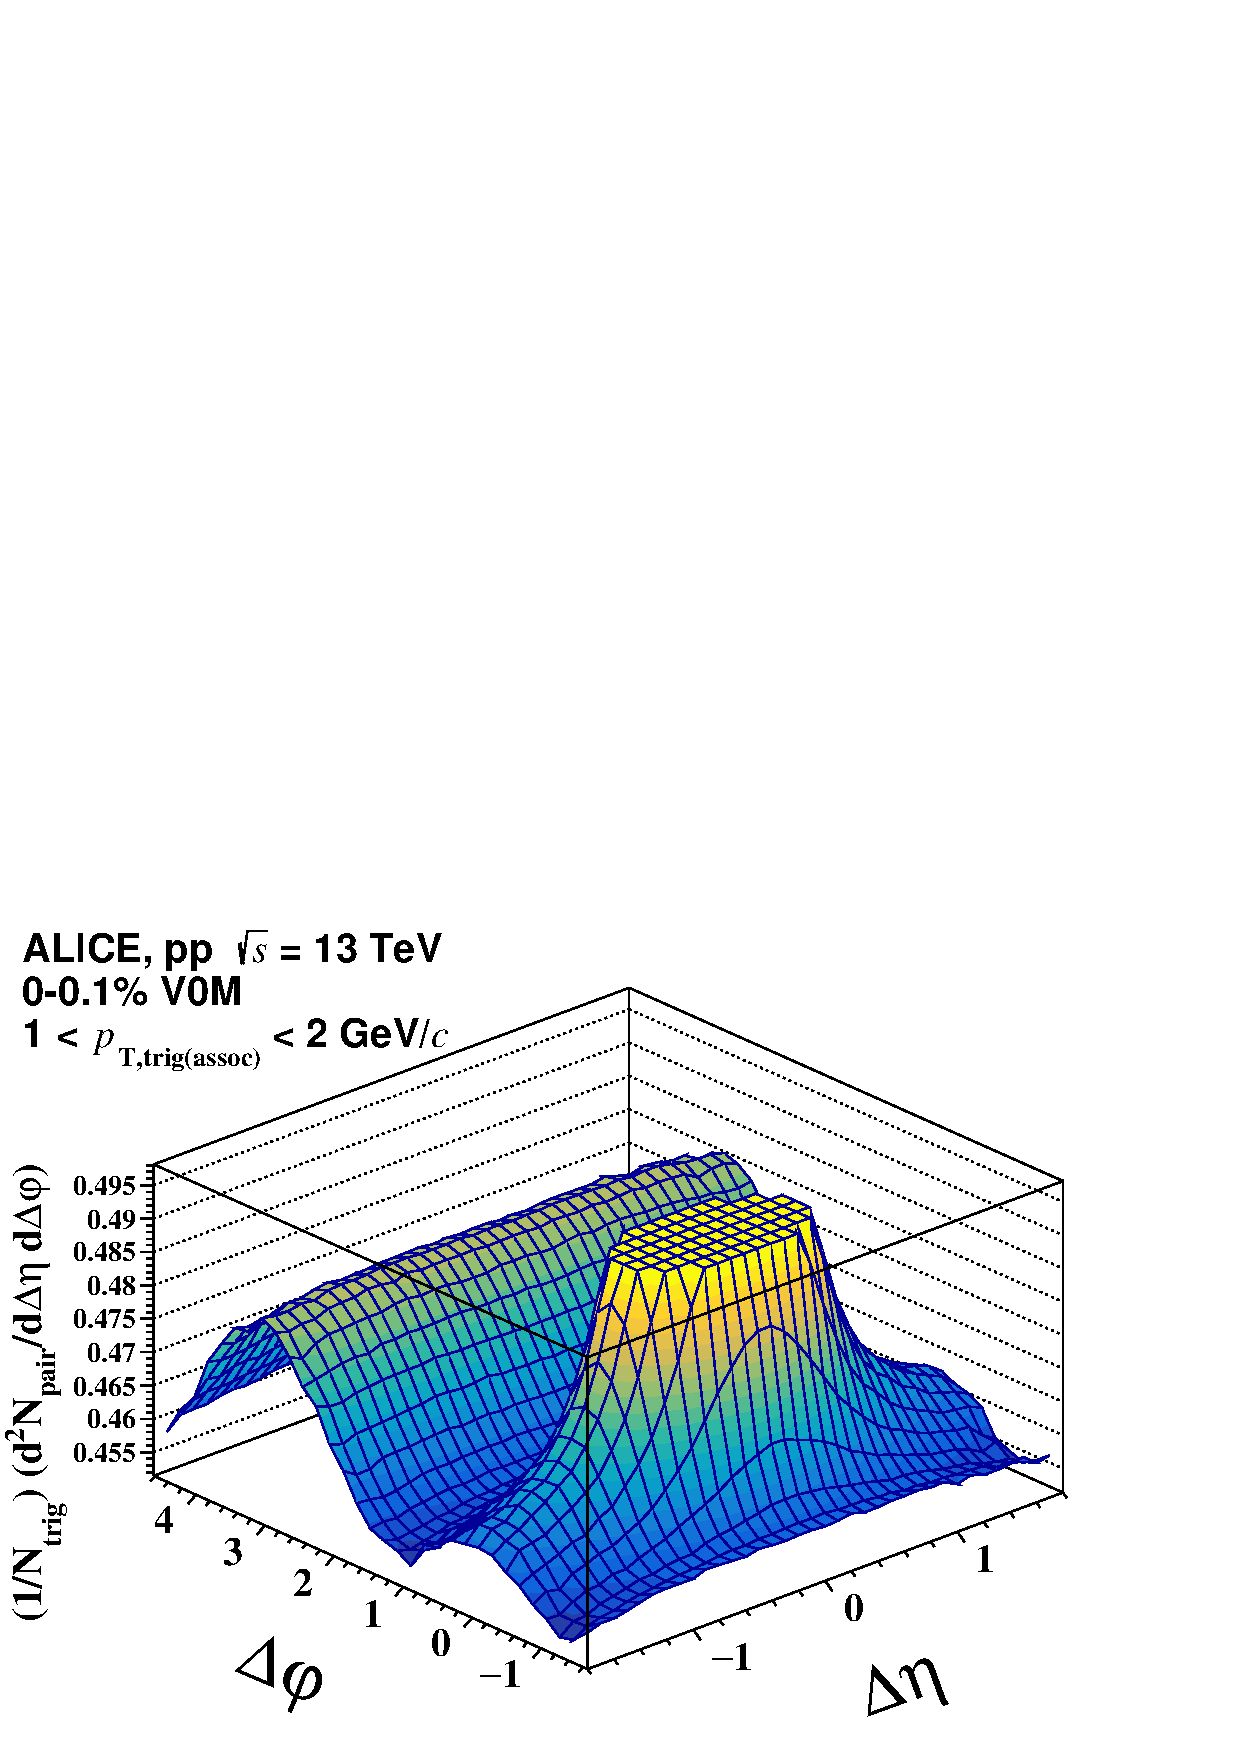
\includegraphics[width=0.4 \textwidth]{./figures/corr1.pdf} }
	\subfigure{ \includegraphics[width=0.4 \textwidth]{./figures/corrmb.pdf} }
	\caption{ Two-dimensional correlations function as function of $\Delta\eta$ and $\Delta\varphi$ in 0-0.1\% (left) and 0-100\% (right) multiplicity class. The interval of transverse momentum of trigger particle and associated particle is 1.0$<\it{p}_{\rm{T}}<$2.0 GeV/\it{c}\rm{}. }
	\label{fig:PlotCorrMBHMT}
\end{figure}

The one-dimensional $\Delta\varphi$ distribution is shown in Fig.~\ref{fig:PlotDeltaPhi} for pairs of particles with various $\it{p}_{\rm{T}}$ intervals in very high multiplicity class. The associated yield per trigger particle is compared with CMS results. The near-side peak is highest in the 1.0$<\it{p}_{\rm{T}}<$2.0 interval and gradually decreases with increasing $\it{p}_{\rm{T}}$.

\begin{figure}[h!]
	\centering
	\includegraphics[width=0.99\linewidth]{./figures/Fig2_PlotDeltaPhi.pdf}
	\caption{One-dimensional $\Delta\varphi$ distribution in the large $\Delta\eta$ with various transverse momentum intervals in each multiplicity class. The distributions in upper panels are measured with 0-100\% multiplicity class. The distribution in lower panels are measured with 0-0.1\% multiplicity class. Interval of transverse momentum of trigger particle and associated particle is 1.0$<\it{p}_{\rm{T}}<$2.0 GeV/\it{c}\rm{} (left), 2.0$<\it{p}_{\rm{T}}<$3.0 GeV/\it{c}\rm{} (middle) and 3.0$<\it{p}_{\rm{T}}<$4.0 GeV/\it{c}\rm{} (right), respectively. }
	\label{fig:PlotDeltaPhi}
\end{figure}
 
The spectra of the ridge yield are shown in Fig.~\ref{fig:PlotYSpect} in very high multiplicity class and compared with CMS results. The estimator of particle multiplicity of ALICE is done with forward subsystem(V0), whereas that of CMS is done by mid-rapidity particles meeting with the condition of $|\eta|<$2.4 and $\it{p}_{\rm{T}}>$0.4 GeV/\it{c}\rm{}. Dedicated comparison is conducted and the difference of particle multiplicity is estimated to be about 20\%. Taking into account the difference in acceptance of charged tracks and comparable definition of multiplicity,, the measurements are can be considered comparable with each other. The spectrum is also compared with model predictions. The PYTHIA8 default and PYTHIA8 + String Shoving are used for the prediction. The PYTHIA8 default is shown as black line and predicts no ridge in pp collisions, which is expected and indicates ignorable jet contamination. The PYTHIA8 + String Shoving is shown as red line and predicts existence of ridge yield in pp collisions, which decreases more rapidly than measurement as transverse momentum increases.

\begin{figure}[h!]
	\centering
	\subfigure{ \includegraphics[width=0.7\textwidth]{./figures/Fig1_RidgeYield.pdf} }
	\caption{ The spectra of ridge yield as function of transverse momentum. The filled circles denote the measurement with ALICE and compared with CMS measurement \cite{ridge_pp_1}, which is represented as open box. The two lines show model predictions from PYTHIA8 default(black line) and PYTHIA8 + String Shoving(red line). }
	\label{fig:PlotYSpect}
\end{figure}

\subsection{Event scale dependent ridge yield}

To further observe the behavior of the ridge yield in events including hard processes, the correlations function is measured with the minimum $\it{p}_{\rm{T, Lead}}$(left) or $\it{p}_{\rm{T, Jet}}$(right) selection for 1.0$<\it{p}_{\rm{T, assoc}},\,\it{p}_{\rm{T, trig}}<$2.0 GeV/\it{c}\rm{}, where the measured ridge yield is maximum in Fig.~\ref{fig:PlotCorrHMTSel}. The ridge structures are still seen with the event scale selection. With the minimum $\it{p}_{\rm{T, Jet}}$ selection, the correlations function has a bump on the $\Delta\eta = 0$ and $\Delta\varphi = \pi$, which occurs due to the limited jet acceptance.

\begin{figure}[h!]
	\centering
	\subfigure{ 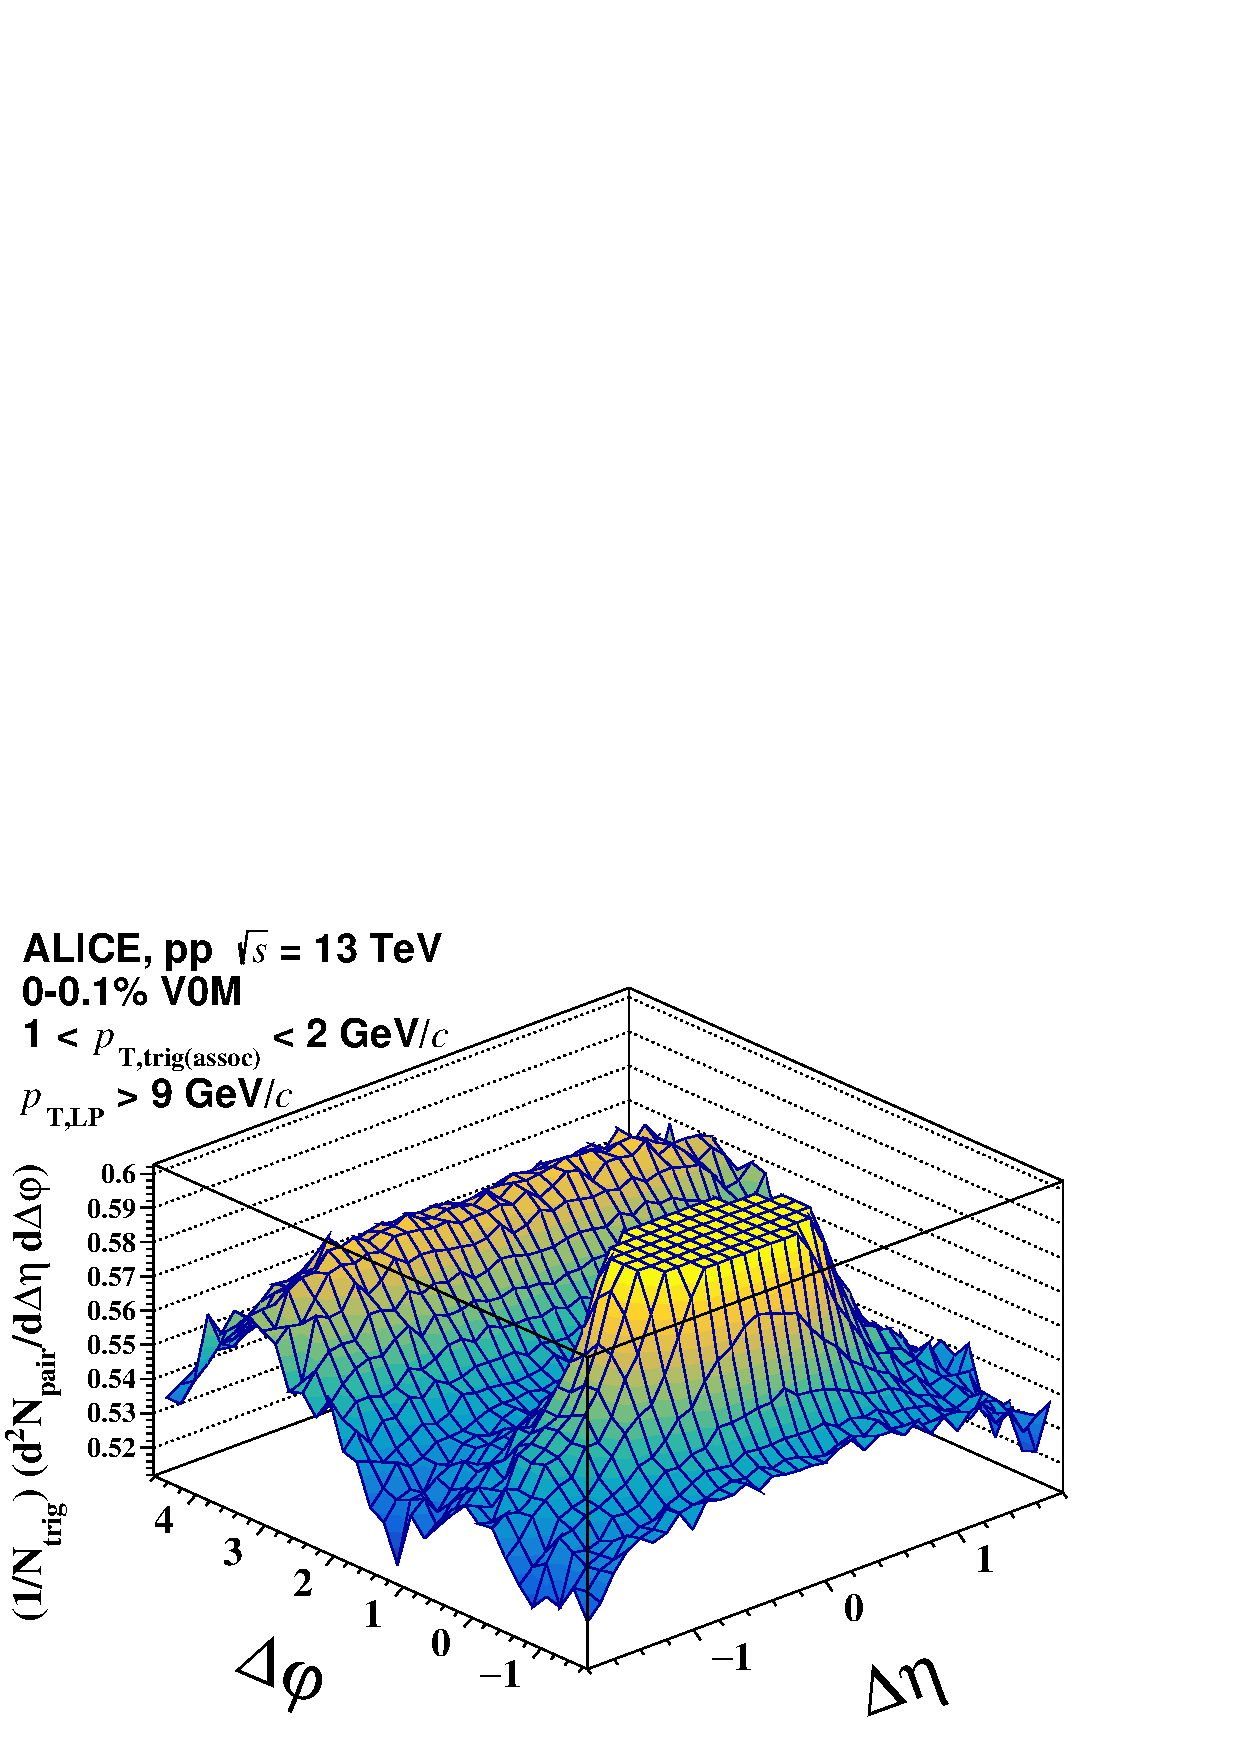
\includegraphics[width=0.4 \textwidth]{./figures/corrlh.pdf} }
	\subfigure{ 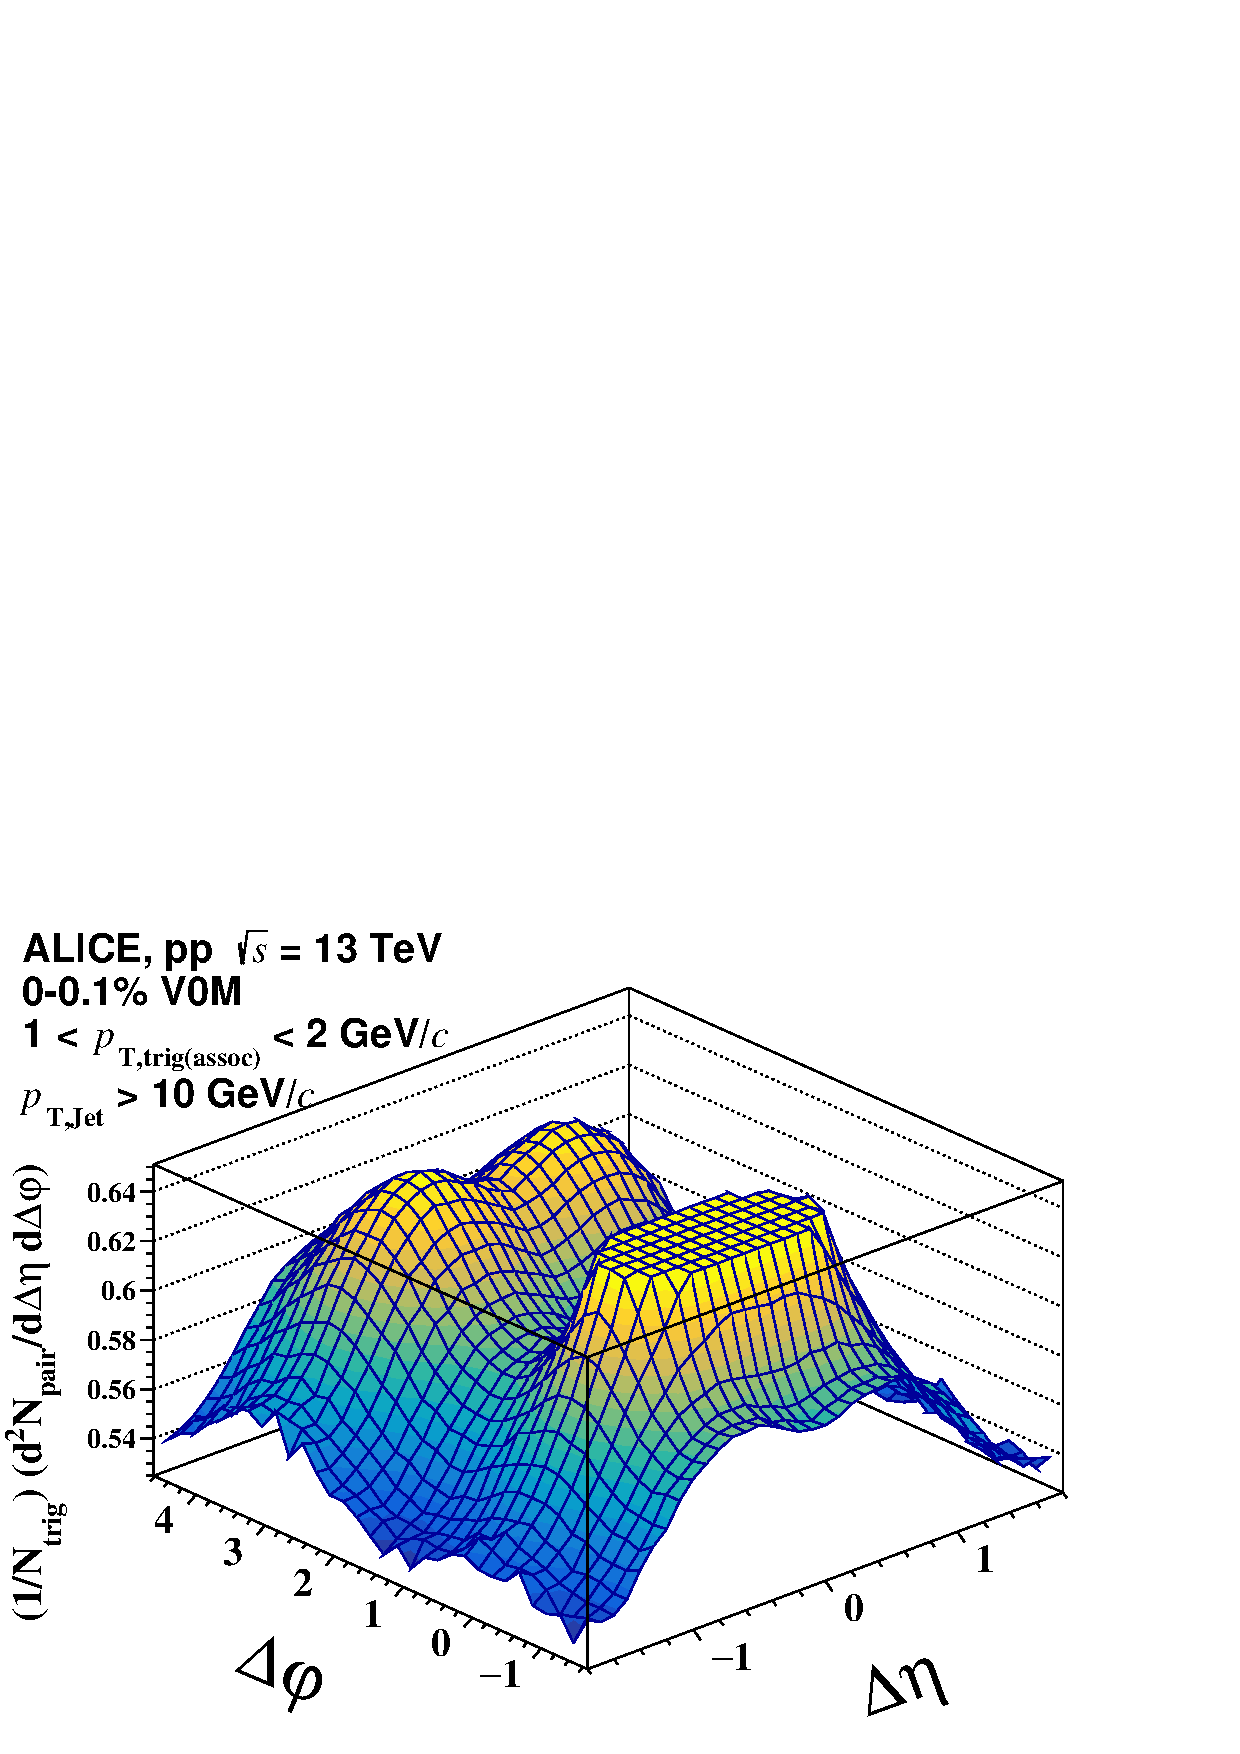
\includegraphics[width=0.4 \textwidth]{./figures/corrjet.pdf} }
	\caption{ Two-dimensional correlations function as function of $\Delta\eta$ and $\Delta\varphi$ in top 0-0.1\% multiplicity class with the minimum $\it{p}_{\rm{T, Lead}}$(left) or $\it{p}_{\rm{T, Jet}}$(right) selection. The interval of transverse momentum of trigger particle and associated particle is 1.0$<\it{p}_{\rm{T}}<$2.0 GeV/\it{c}\rm{}. The minimum requirement for $\it{p}_{\rm{T, Lead}}$ or $\it{p}_{\rm{T, Jet}}$ is 9 GeV/\it{c}\rm{} or 10 GeV/\it{c}\rm{}, respectively. }
	\label{fig:PlotCorrHMTSel}
\end{figure}

The one-dimensional $\Delta\varphi$ distribution with the minimum $\it{p}_{\rm{T, Lead}}$(left) or $\it{p}_{\rm{T, Jet}}$ is shown in Fig.~\ref{fig:PlotDeltaPhiESE}. The near-side yield increases as the event scale increases by requiring higher $\it{p}_{\rm{T, Lead}}$(left) or $\it{p}_{\rm{T, Jet}}$. The model comparisons are seen as blue line for PYTHIA8 + String Shoving and apricot line for PYTHIA8 default, respectively. The PYTHIA8 + String Shoving describes ridge yield with the selection. The PYTHIA8 default predict the ridge yield to be zero with the selection, which also tell there is little ignorable jet contamination. Both models well describe the away-side yield with the $\it{p}_{\rm{T, Jet}}$ selection and overestimates away-side yield with the $\it{p}_{\rm{T, Lead}}$ selection.

\begin{figure}[h!]
	\centering
	\includegraphics[width=0.99\linewidth]{./figures/Fig5_PlotDeltaPhiESE.pdf}
	\caption{ One-dimensional $\Delta\varphi$ distribution in the large $\Delta\eta$ with the minimum $\it{p}_{\rm{T, Lead}}$(lower) or $\it{p}_{\rm{T, Jet}}$(upper) selection for 1.0$<\it{p}_{\rm{T, assoc}},\,\it{p}_{\rm{T, trig}}<$2.0 GeV/\it{c}\rm{} in 0-0.1\% multiplicity class. The filled circles show measurement with ALICE. Model predictions are compared with measurement as blue line for PYTHIA8 + String Shoving  and apricot line for PYTHIA8 default.}
	\label{fig:PlotDeltaPhiESE}
\end{figure}

The spectra of the ridge yield as function of the minimum $\it{p}_{\rm{T, Lead}}$(left) or $\it{p}_{\rm{T, Jet}}$(right) are shown in Fig.~\ref{fig:RidgeYield_ESE}. The spectra are compared with model predictions. 
The increases of ridge yield with the selections are observed and the model with PYTHIA8 + String Shoving underestimates the ridge yield. with the $\it{p}_{\rm{T, Jet}}$ selection. the model prediction with PYTHIA8 default still assures ignorable jet contamination.

\begin{figure}[h!]
	\centering
	\includegraphics[width=0.99\linewidth]{./figures/Fig6_RidgeYieldESE.pdf}
	\caption{The ridge yield spectra with respect to the leading particle and jet selections. The filled circles show measurement with ALICE. Model predictions are compared with measurement as blue line for PYTHIA8 + String Shoving  and apricot line for PYTHIA8 default.}
	\label{fig:RidgeYield_ESE}
\end{figure}



